\documentclass{article}
\usepackage{graphicx} % Required for inserting images
\usepackage{wrapfig}
\usepackage{hyperref}
\usepackage[export]{adjustbox}
\usepackage{geometry}
\setcounter{secnumdepth}{5}
\setcounter{tocdepth}{5}
\geometry{a4paper,
 total={170mm,257mm},
 left=5mm,
 top=20mm}

\title{Gruppo C (Federico, Antonio, Miri, Elena)}
\author{Giovanni Cisternini}
\date{December 2023}

\begin{document}
\tableofcontents


\section{NPC}

    \subsection{Animali}
   
        
           
            \begin{tabular}{|c|c|c|}
                \hline 
                \hypertarget{doberman}{Doberman} & \hypertarget{granchio}{Granchio Gigante} & \hypertarget{uomorana}{Uomorana}\\ 
                \includegraphics[width=4cm, height = 6 cm]{../Mostri/Doberman.png}  &\includegraphics[width=4cm, height = 6 cm]{../Mostri/Granchio Gigante.PNG} &  \includegraphics[width=4cm, height = 6 cm]{../Mostri/Bullywug.PNG}\\
                \hline
                \hypertarget{lupo}{Lupo} & Salamandra & \hypertarget{re}{ReDeiRospi} \\ 
                \includegraphics[width=4cm,height=6cm]{../Mostri/Lupo.png} & \includegraphics[width=4cm, height = 6 cm]{../Mostri/Mastino.PNG} & \includegraphics[width=4cm, height = 6 cm]{../Mostri/ReDeiRospi.PNG} \\
                \hline
                \hypertarget{sciame}{Sciame Di Quipper} & \hypertarget{Orsogufo}{Orsogufo} \\  
                \includegraphics[width=4cm, height = 6 cm]{../Mostri/Sciame di Quippers.PNG} &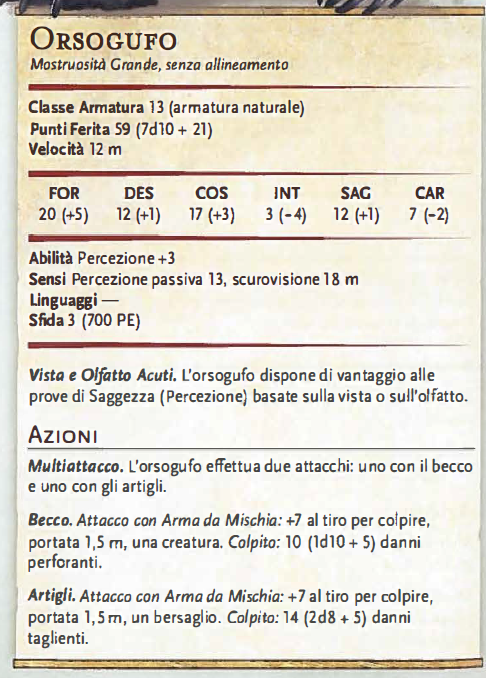
\includegraphics[width=4cm,height = 6cm]{../Mostri/Orsogufo.png} \\
                \hline 
                
            \end{tabular}
       
    \subsection{Mostri}
    \newpage
    
       
       
        \begin{tabular}{|c|c|c|}
            \hline
            \hypertarget{bandito}{Bandito} & \hypertarget{kenk}{Kenku} &  \hypertarget{troll}{troll} \\
            \includegraphics[width=4cm, height = 6 cm]{../Mostri/Bandito.PNG} & \includegraphics[width=4cm, height = 6 cm]{../Mostri/Kenku.PNG} & \includegraphics[width=4cm, height = 6 cm]{../Mostri/Troll.PNG}\\
            \hline
            \hypertarget{malvivente}{Malvivente(YARGA)} & \hypertarget{orco}{Orco}  & Mago \\
            \includegraphics[width=4cm, height = 6 cm]{../Mostri/Malvivente.PNG} & \includegraphics[width=4cm, height = 6 cm]{../Mostri/Orco.PNG} &  \includegraphics[width=4cm, height = 6 cm]{../Mostri/mago.png}\\
            \hline
            \hypertarget{goblin}{Goblin}&  \hypertarget{Iarno}{Iarno} & \hypertarget{zombi}{Zombi}  \\
            \includegraphics[width=4cm,height=6cm]{../Mostri/Goblin.png}& \includegraphics[width=4cm,height = 6cm]{../Mostri/HalmunKost.png} & \includegraphics[width=4cm,height = 6cm]{../Mostri/Zombi.png}\\
            \hline

        \end{tabular}
        \newpage
        \begin{tabular}{|c|c|c|}         
            \hline
             \hypertarget{uccello}{Uccello Stigeo}&  \hypertarget{nothic}{Nothic} & \hypertarget{scheletro}{Scheletro} \\
             \includegraphics[width=4cm,height = 6cm]{../Mostri/UccelloStigeo.png}& \includegraphics[width=4cm,height = 6cm]{../Mostri/Nothic.png}&\includegraphics[width=4cm,height = 6cm]{../Mostri/Scheletro.png}\\
            \hline
            \hypertarget{marchirossi}{Marchi Rossi}  & \hypertarget{ogre}{Ogre}& Bugbear\\
            \includegraphics[width=4cm,height = 6cm]{../Mostri/Marchi Rossi.PNG} & \includegraphics[width=4cm,height = 6cm]{../Mostri/Ogre.png}  & \includegraphics[width=4cm,height = 6cm]{../Mostri/Bugbear.png}\\
            \hline
            \hypertarget{gnoll}{Gnoll Hunter}&  \hypertarget{gnoll}{Gnoll} & \hypertarget{gnoll}{Gnoll Flesh} \\
            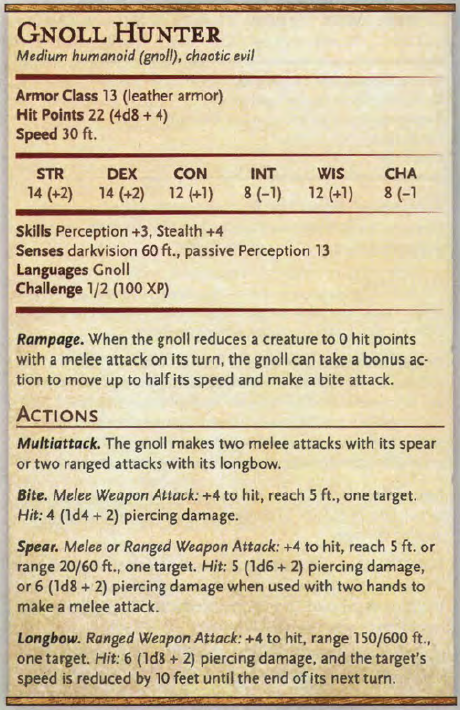
\includegraphics[width=4cm,height = 6cm]{../Mostri/Gnoll_Hunter.png}& 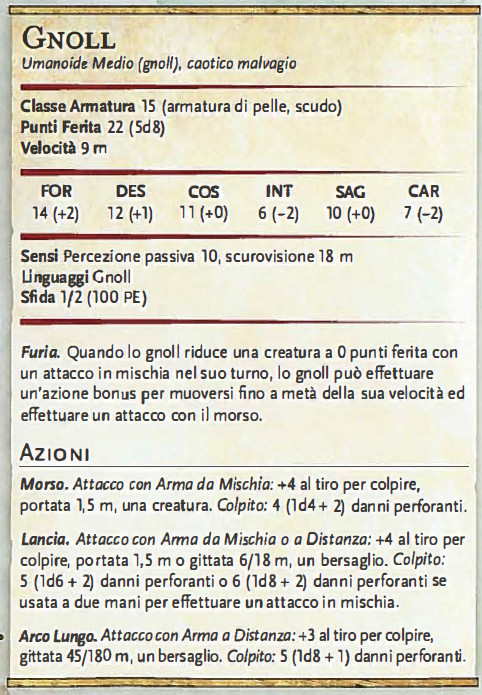
\includegraphics[width=4cm,height = 6cm]{../Mostri/Gnoll.png}&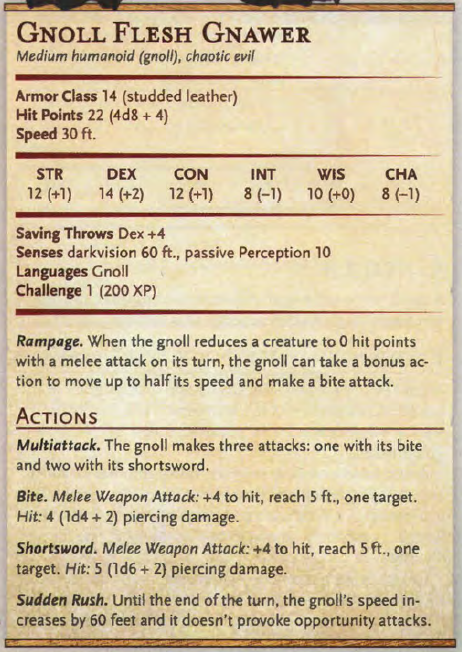
\includegraphics[width=4cm,height = 6cm]{../Mostri/Gnoll_Flesh.png}\\
            \hline
        \end{tabular}     
        \newpage   
        \begin{tabular}{|c|c|c|}
            \hline
            \hypertarget{gnoll}{Gnoll Lord}&  \hypertarget{gnoll}{Gnoll Zanna} & \hypertarget{Centauro}{Centauro} \\
            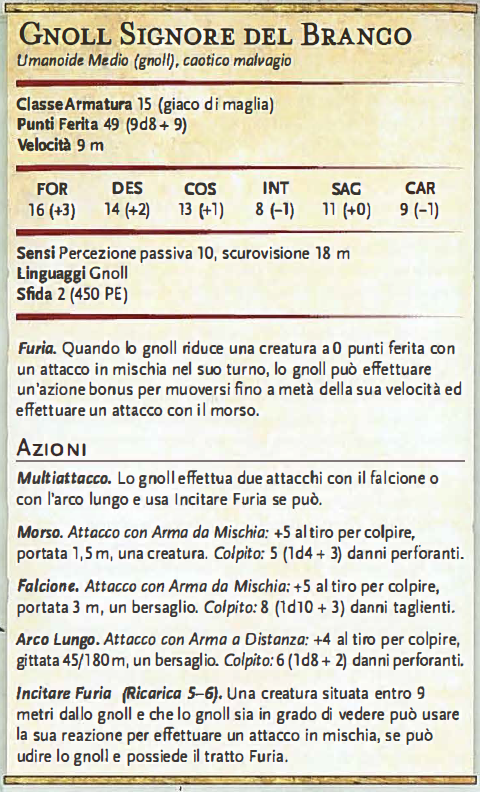
\includegraphics[width=4cm,height = 6cm]{../Mostri/Gnoll_lord.png}& 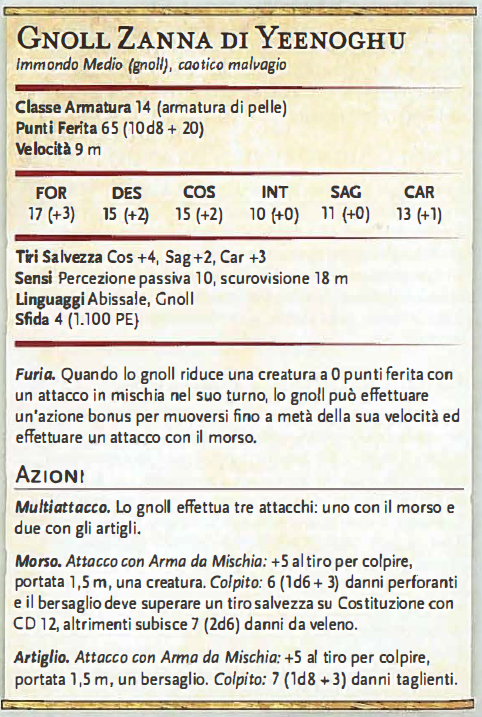
\includegraphics[width=4cm,height = 6cm]{../Mostri/Gnoll_Zanna.png}&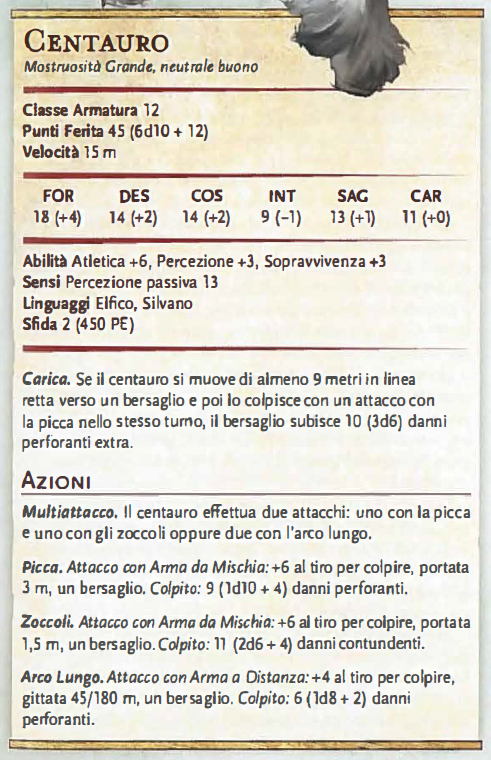
\includegraphics[width=4cm,height = 6cm]{../Mostri/Centauro.png}\\
            \hline
            \hypertarget{hobgoblin}{Hobgoblin}& \hypertarget{hobgoblin}{Ghoul} &\hypertarget{hobgoblin}{Scheletri}\\
            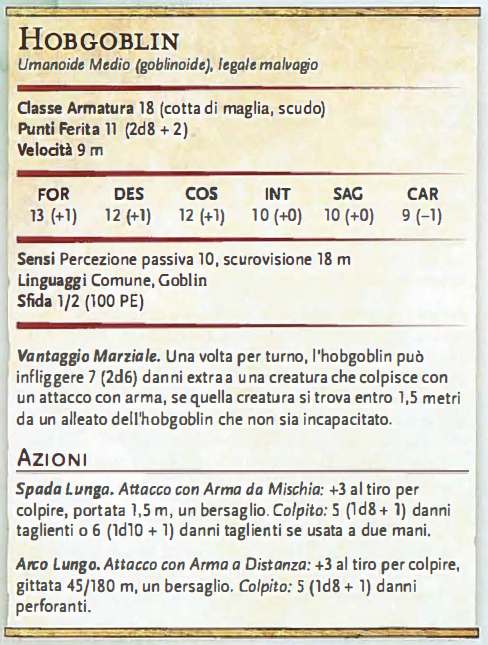
\includegraphics[width=4cm,height = 6cm]{../Mostri/Hobgoblin.png} &   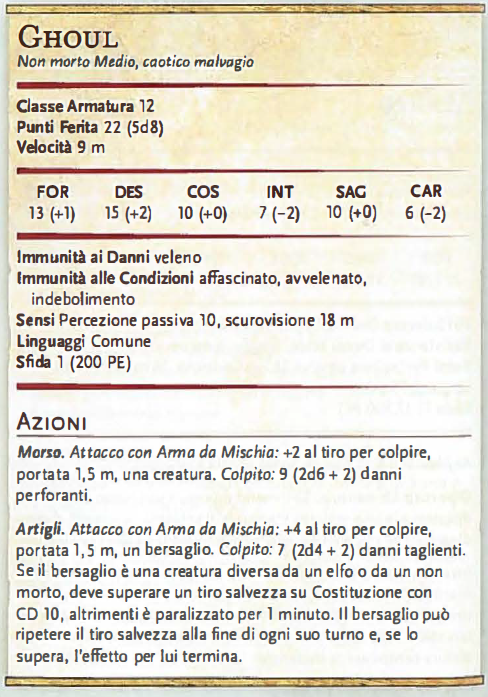
\includegraphics[width=4cm,height = 6cm]{../Mostri/Ghoul.png} &   \includegraphics[width=4cm,height = 6cm]{../Mostri/Scheletro.png}\\
            \hline
            \hypertarget{grick}{Grick}& \hypertarget{ameba}{Ameba\_paglierina} &\hypertarget{zombi}{Zombie}\\
            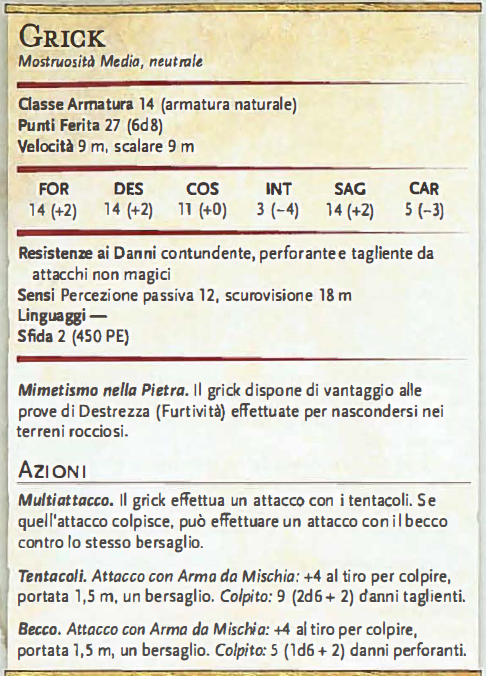
\includegraphics[width=4cm,height = 6cm]{../Mostri/Grick.png} &   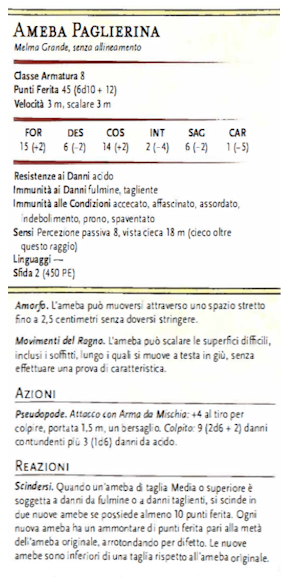
\includegraphics[width=4cm,height = 6cm]{../Mostri/ameba_paglierina.png} &   \includegraphics[width=4cm,height = 6cm]{../Mostri/Zombi.png}\\
        \end{tabular} 
   
    \subsection{Alleati o Personaggi}
    \newpage


   
    \begin{tabular}{|c|c|c|}
        \hline
        \hypertarget{Duran}{Duran} & \hypertarget{Xoblob}{Xoblob} & \hypertarget{guardia}{Guardia}  \\
        \includegraphics[width=4cm, height = 6 cm]{../PNG/Duran.png} &  \includegraphics[width=4cm, height = 6 cm]{../Mostri/Gnomo_delle_profondita.png} &\includegraphics[width=4cm, height = 6 cm]{../Mostri/Guardia.png} \\
        \hline
        \hypertarget{Reaner}{Reaner} & \hypertarget{sildar}{Sildar} & \hypertarget{VigilanzaS}{Vigilanza\_Cittadina\_Sup} \\
        \includegraphics[width=4cm, height = 6 cm]{../PNG/Reaner_Nevember_Spadaccino.png}&\includegraphics[width=4cm,height=6cm]{../PNG/Sildar_Hallwinter.png} &  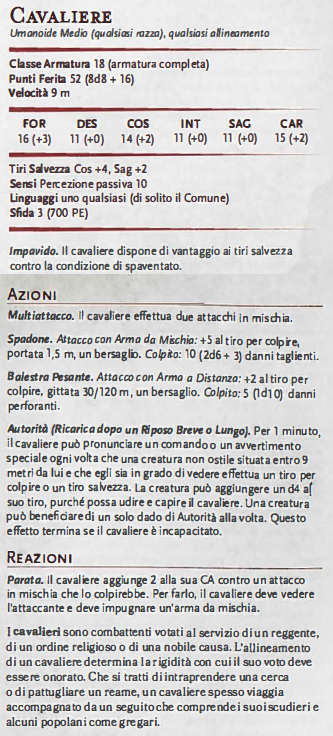
\includegraphics[width=4cm, height = 6 cm]{../Mostri/Cavaliere.png}\\
       
         
        \hline
        \hypertarget{GuardiaB}{Guardia\_Cittadina\_Base} & \hypertarget{GuardiaT}{Guardia\_Cittadina\_Tenente} & \hypertarget{VigilaB}{Vigilanza\_Cittadina\_Base } \\
        (Soldato o Sergente)&( Tenente, Capitano o più su)&(quasi tutti, randelli elmi) \\
        \includegraphics[width=4cm, height = 6 cm]{../Mostri/Guardia.png} & 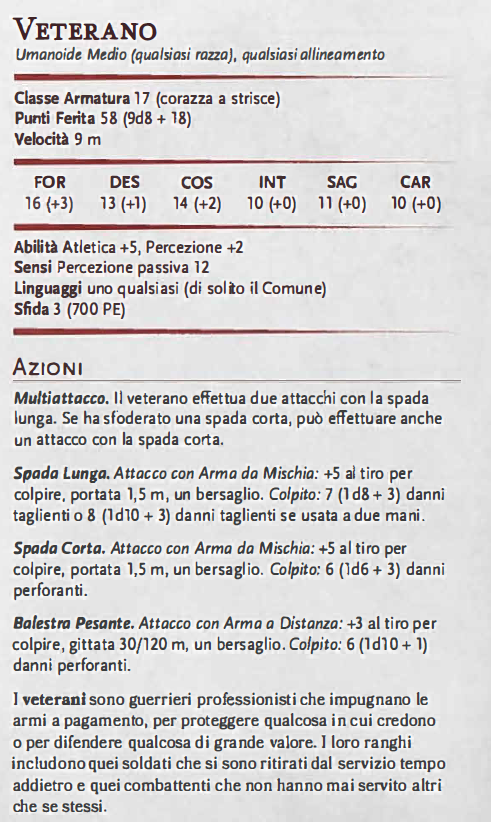
\includegraphics[width=4cm, height = 6 cm]{../Mostri/Veterano.png} & 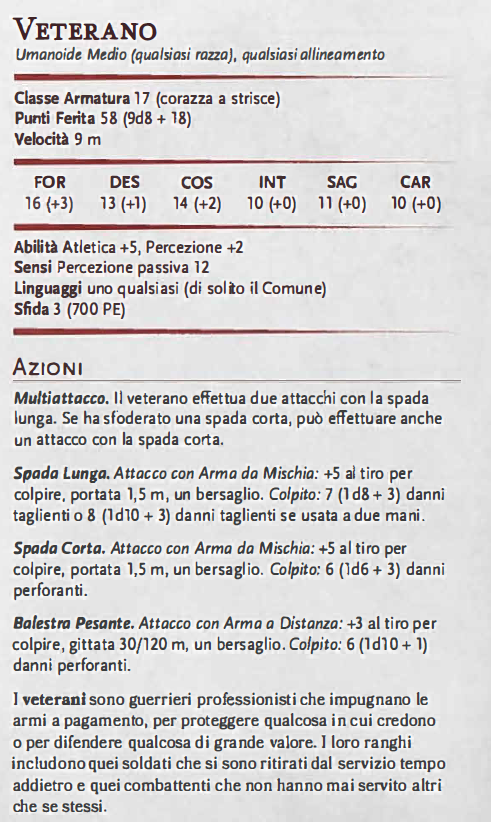
\includegraphics[width=4cm, height = 6 cm]{../Mostri/Veterano.png} \\
        
         \hline
    \end{tabular}







\section{Trama}



\subsection{Cammino di resurrezione}
Vidar dopo aver nascosto il suo amico in una casa a confini della campagna di Waterdeep, entra nella città e chiede informazioni, entra in una taverna e chiede se conosce qualche luogo in cui il culto tratti della resurrezione, il locandiere non sa nulla di culti, allora Vidar cerca di capire se ci sono templi in generale, viene allora indirizzato verso Il tempio della natura dove non ha una risposta ben precisa ma gli viene detto che sicuramente alla Fonte della Conoscenza avrebbe trovato le informazioni che cercava. 
\paragraph{Fonte della Conoscenza}
    \subparagraph{Descrizione} ... già fatta.

  
    \subparagraph{Descrizione della Grande Biblioteca}
    La Grande Biblioteca del Legatore, situata nel tempio Fonte della Conoscenza di Waterdeep, è una maestosa struttura che si estende su quattro piani interi. Questa biblioteca è dedicata alla preservazione e alla diffusione della conoscenza e funge da importante centro per studiosi, maghi e sacerdoti.
    
    All'interno della biblioteca, un ampio e silenzioso scriptorium è destinato alla scrittura e alla copia dei manoscritti. Qui, scribi e copisti lavorano diligentemente per trascrivere testi antichi e creare nuove opere. Le pareti della biblioteca sono rivestite di scaffali colmi di libri, pergamene e tomi rari, coprendo una vasta gamma di argomenti, dalle arti arcane alla storia, dalla filosofia alla teologia.
    
    Ogni piano della biblioteca è accessibile tramite eleganti scalinate di legno e balconi che si affacciano sui livelli inferiori, offrendo una vista panoramica dell'intera collezione. La luce naturale filtra attraverso le vetrate colorate, illuminando delicatamente gli spazi di lettura e studio.
    
    La Grande Biblioteca del Legatore non è solo un deposito di conoscenza, ma anche un luogo di apprendimento e contemplazione, dove i visitatori possono esplorare il vasto patrimonio intellettuale e spirituale di Waterdeep.
    
    \subparagraph{Incontro Aria Whucknolls:} 
        Chiedendo in giro (se urla viene zittito), alcuni fanno riferimento ad Aria Whucknolls come la più adatta rispondere a suoi quesiti, lo invitano a cercare nella sezione Culti e Religioni. La trova china su un libro a studiare immersivamente. 

        \subparagraph{Descrizione di Aria Whucknolls}
        Aria Whucknolls è una rispettata bibliotecaria presso la Grande Biblioteca del Legatore nel tempio Fonte della Conoscenza di Waterdeep. Con una profonda conoscenza delle religioni e delle divinità umane, Aria è una figura chiave nella gestione e nell'ordinamento dei testi sacri e dei documenti storici relativi alle credenze spirituali.
        
        Fisicamente, Aria è una donna di mezza età con una statura media e una corporatura snella. Ha capelli castani raccolti in un'elegante acconciatura, che lascia intravedere qualche filo d'argento, e occhi penetranti color nocciola che riflettono la sua intelligenza e curiosità. Porta spesso occhiali da lettura sottili che poggiano delicatamente sul ponte del naso. Il suo abbigliamento è semplice ma dignitoso, solitamente composto da abiti lunghi e modesti nelle tonalità del blu e del grigio, che si addicono al suo ruolo di custode della conoscenza.
        
        Comportamentalmente, Aria è conosciuta per la sua pazienza e il suo approccio metodico. La sua presenza è sempre accogliente e rassicurante, rendendo la biblioteca un luogo di rifugio e studio per chiunque cerchi sapere. È una persona tranquilla e riflessiva, dotata di una grande capacità di ascolto e di un'attitudine gentile verso tutti. Nonostante la sua natura riservata, Aria è sempre disponibile a condividere la sua vasta conoscenza con chi ne ha bisogno, tenendo occasionali lezioni e conferenze sulla teologia.
        
        Oltre alle sue mansioni di bibliotecaria, Aria è nota per la sua passione per la conoscenza e la sua dedizione alla ricerca, rendendola una guida preziosa per chiunque sia interessato alle religioni e alle divinità. La sua sorella, Cera, è un pilastro nella sua vita. Nonostante le loro vite possano seguire percorsi diversi, la connessione tra Aria e Cera è un punto fermo nella vita di entrambe, supportandosi reciprocamente nelle sfide e nei successi.
    
    \subparagraph{Libri procurati da Aria} \begin{itemize}
        \item \textit{Gli Dei e i Mortali: Un Viaggio attraverso il Pantheon di Faerûn} (Informazion Su Lathander)
        \item \textit{Le Leggende di Oghma: Racconti di Sapienza e Conoscenza}
        \item \textit{Il Sentiero dei Druidi: Silvanus e i Guardiani della Natura}
        \item \textit{Le Cronache di Mystra: La Magia Divina e i Suoi Seguaci}
        \item \textit{Il Codice di Helm: La Giustizia e i Paladini dell'Ordine}
    \end{itemize}

\subparagraph{Lathander e il Suo Culto}
Lathander, conosciuto anche come l'Alba Radiosa, è una delle divinità più venerate nei Forgotten Realms. È il dio dell'alba, della nascita, della rinascita, della vitalità e della creatività. Lathander è spesso associato al sole nascente e simboleggia nuovi inizi, speranza e prosperità. Il suo dominio include anche la giovinezza e la primavera, rappresentando la promessa di un nuovo giorno e di nuove possibilità.

\subparagraph{Descrizione Fisica e Simbolismo}
Lathander è spesso raffigurato come un uomo alto e imponente, con lunghi capelli dorati e occhi scintillanti che emanano una luce calda e confortante. Indossa abiti ricchi e luminosi, spesso in tonalità dorate e rosse, che simboleggiano il sole nascente. Il suo simbolo più riconosciuto è un sole splendente, spesso rappresentato con raggi dorati che si estendono in tutte le direzioni.

\subparagraph{Il Culto di Lathander}
Il culto di Lathander è diffuso in tutto il Faerûn, con molti seguaci che venerano il dio nelle terre civilizzate e rurali. I chierici e i paladini di Lathander sono noti come "Lathanderiti" e sono dedicati a promuovere i valori della loro divinità attraverso atti di bontà, coraggio e rinnovamento. Essi spesso guidano cerimonie all'alba, dove pregano per la benedizione di Lathander e chiedono la sua guida per il giorno a venire.

\subparagraph{Templi e Cerimonie}
I templi dedicati a Lathander sono magnifici e spesso situati in luoghi dove la vista dell'alba è particolarmente spettacolare. Questi templi sono decorati con simboli solari, vetrate colorate e statue che rappresentano Lathander e le sue virtù. Le cerimonie del culto di Lathander sono solitamente tenute all'alba, con preghiere, canti e offerte fatte mentre il sole sorge. Questi rituali sono volti a celebrare la luce e a chiedere la benedizione di Lathander per prosperità e protezione.

\subparagraph{Insegnamenti e Dogmi}
Lathander insegna ai suoi seguaci l'importanza del rinnovamento e del cambiamento positivo. Egli promuove l'ottimismo e la speranza, incoraggiando i suoi fedeli a vedere ogni giorno come una nuova opportunità per fare del bene. La distruzione delle forze del male, la cura dei malati e la protezione dei deboli sono tra i principali doveri dei Lathanderiti. Inoltre, Lathander spinge i suoi seguaci a essere creativi e a cercare sempre di migliorare se stessi e il mondo intorno a loro.

\subparagraph{Festività}
Una delle festività più importanti del culto di Lathander è il "Giorno della Semina", celebrato in primavera. Durante questa festività, i seguaci piantano nuovi raccolti, simbolizzando la promessa di una nuova vita e prosperità. Un'altra celebrazione significativa è il "Festival dell'Alba", che si tiene all'inizio dell'anno, durante il quale si celebrano nuovi inizi e si riflette sull'anno passato.

In sintesi, Lathander e il suo culto rappresentano la speranza, la rinascita e il potenziale di ogni nuovo giorno. I suoi seguaci lavorano instancabilmente per diffondere luce e bontà nel mondo, ispirati dall'esempio luminoso della loro divinità.

\paragraph{Guglie del mattino}
            \subparagraph{Descrizione delle Guglie del Mattino}

            \subparagraph{Esterno}
            Le Guglie del Mattino sono una maestosa cattedrale dedicata a Lathander, situata in un'area dove la prima luce dell'alba può essere apprezzata in tutto il suo splendore. Costruita interamente in marmo rosa, questa struttura a tre piani emana una calda luminosità naturale che risplende sotto il sole nascente. La cattedrale è sormontata da sette guglie, ciascuna realizzata in metalli preziosi: rame, oro e argento. Queste guglie brillano magnificamente quando i primi raggi del sole le colpiscono, riflettendo la gloria dell'alba e creando uno spettacolo di luce che incanta i fedeli e i visitatori.
            
            \subparagraph{Interno}
            All'interno, le Guglie del Mattino sono altrettanto impressionanti. L'ingresso principale conduce a una vasta navata, con alti soffitti e colonne di marmo rosa che si ergono maestosamente. La luce del mattino penetra attraverso le vetrate colorate che adornano le pareti, proiettando un arcobaleno di colori sul pavimento e sulle superfici circostanti. Queste vetrate raffigurano scene della vita di Lathander, episodi di rinnovamento e vittoria della luce sull'oscurità.
            
            Il cuore della cattedrale è il grande altare, realizzato in oro e decorato con intarsi di argento e rame. Dietro l'altare, una grande finestra circolare incornicia il sole nascente, simbolo della benedizione continua di Lathander sul suo popolo. Lungo le navate laterali si trovano cappelle più piccole dedicate a diverse virtù e aspetti di Lathander, ciascuna con il proprio altare e decorazioni specifiche.
            
            Al secondo piano, accessibile tramite scale larghe e maestose, si trova la biblioteca del tempio, una sala tranquilla dove i sacerdoti e gli studiosi possono studiare i testi sacri e riflettere sugli insegnamenti di Lathander. Il terzo piano ospita sale di meditazione e preghiera, spazi tranquilli e sereni dove i fedeli possono trovare pace e ispirazione.
            
            Le Guglie del Mattino non sono solo un luogo di culto, ma anche un centro comunitario, dove si tengono regolarmente cerimonie, feste e riunioni che rafforzano il legame tra i seguaci di Lathander. La cattedrale è un simbolo di speranza e rinascita, riflettendo in ogni dettaglio la missione del dio dell'alba di portare luce e rinnovamento al mondo.
            
            \subparagraph{Parlare con Chierici a Caso} La maggior parte dei chierici sono ex militanti e soldati di basso livello, quasi tutti molto cordiali e disponibili, non sanno molto su possibili tecniche di Ressurezione, ma sono conviti che l'Alta Radiosità Ghentilara o il Priore Athosar possano essere d'aiuto. 

            \subparagraph{Parlare con Athosar} 
            \textbf{Descrizione Ghentilara: } Ghentilara è una mezzelfa di straordinaria bellezza e grazia, che incarna perfettamente l'eleganza e la saggezza mescolate alle sue origini elfiche e umane. La sua carnagione è liscia e di un tono olivastra, rispecchiando la sua eredità elfica, mentre i suoi lunghi capelli intrecciati, un tempo scuri, sono ora splendenti di un bianco argenteo, testimonianza dei secoli di vita che ha vissuto.

            Come molte mezzelfe, Ghentilara possiede lineamenti affascinanti e occhi profondi, che trasmettono una combinazione di calma e risolutezza. La sua figura è slanciata e elegante, con movimenti che riflettono una grazia naturale. Indossa abiti che combinano la praticità della vita quotidiana con l'eleganza delle sue occasioni più formali, sempre scegliendo tessuti di qualità e colori che esaltano la sua bellezza senza ostentazione.
            
            Oltre alla sua presenza fisica, Ghentilara possiede un'intelligenza acuta e una profonda compassione, caratteristiche che sono tipiche delle mezzelfe che hanno abbracciato appieno entrambe le metà della loro eredità. È in grado di navigare con maestria attraverso una varietà di situazioni e ambienti, sia nelle attività quotidiane con i contadini della sua comunità, sia negli intrighi politici e nei negoziati con altri dignitari. Il suo approccio equilibrato e la sua capacità di mediare tra diversi punti di vista sono apprezzati da tutti coloro che hanno il privilegio di lavorare con lei.
            
            Ghentilara è una figura rispettata e ammirata nella sua comunità, una guida sia per la sua saggezza che per il suo impegno nel migliorare la vita di coloro che la circondano. La sua presenza è un faro di speranza e stabilità per chiunque incontri nel suo cammino.\\

                  \textbf{Cosa sa:} Athosar ovviamente sa che nella sua religione si pratica la resurrezione, ma è convinta che bisogna meritarsela (CD 12 Persuasione) : farà domande sulle motivazioni che spingono Vidar a voler resuscitare l'amico e chiederà informazioni riguardo l'amico. Se viene persuasa darà informazioni riguardo all'incatesimo cercato, spiegando però che i chierici in grado di eseguire quell'incantesimo sono rarissimi e lei ne conosce solo uno ( Alta Radiosità Ghentilara ), ma che non sa dove si trovi di preciso, sa solo che si stava dirigendo verso le Montagne del Tramonto per un ritiro. 
                    \\
                  \textbf{Descrizione di Athoras, Priore della Chiesa delle Guglie del Mattino}
                  Athoras è un uomo di profonda devozione e leadership all'interno della Chiesa delle Guglie del Mattino, dedicata al culto di Lathander, il dio dell'alba. Di media statura e corporatura robusta, Athoras porta con fierezza la sua carica di priore con un atteggiamento serio ma compassionevole. La sua pelle è leggermente abbronzata, segno della sua vita trascorsa sotto il sole dell'alba, mentre i suoi capelli corti sono di un castano scuro ormai grigio per via degli anni di servizio e saggezza acquisiti.
                  
                  Athoras veste l'abito cerimoniale della Chiesa delle Guglie del Mattino, composto da tunica bianca con ricami dorati che simboleggiano il sole nascente, e un mantello rosso intenso che rappresenta la passione e la devozione nel servire Lathander. Porta sempre con sé il simbolo sacro del dio, un sole splendente, appeso a una catenella d'oro intorno al collo.
                  
                  Come priore, Athoras è noto per la sua capacità di ispirare e guidare i suoi fedeli. Le sue prediche sono eloquenti e motivanti, enfatizzando i valori di speranza, rinascita e prosperità che Lathander incarna. È rispettato non solo per la sua conoscenza teologica, ma anche per la sua capacità di ascolto e il suo approccio compassionevole nei confronti di chi cerca conforto e guida spirituale.
                  
                  Nel tempo libero, Athoras dedica tempo alla meditazione e alla preghiera personale, cercando di approfondire il suo legame con Lathander e rinnovare il suo spirito per meglio servire la sua comunità. È un leader rispettato non solo all'interno della chiesa, ma anche nella comunità circostante, dove si impegna attivamente nel migliorare le condizioni di vita dei suoi fedeli e promuovere l'armonia sociale.
                  
                  Athora incarna l'ideale del sacerdote guerriero di Lathander, che combina la forza fisica con la compassione spirituale, servendo come esempio vivente dei principi della sua fe
    \subsubsection{Viaggio verso le Montagne del Tramonto}
       
        Dopo aver parlato con Athoras, Vidar assieme al suo accompagnatore Necrov, devono decidere se andare a piedi o con una carrozza, il chierico suggerisce di andare in carrozza perché il viaggio è lungo, quindi lo dirige verso la porta Sud verso la casa del Puledro, dove vi è un umano di nome Arman che vende e noleggia corrozze. Putroppo però la giornata è quasi finita, e gli è rimasto un ultimo carro e un solo cavallo. In contemporanea ai due arriva anche una giovane Tielfing, anche lei in cerca di un carretto che le serve per viaggiare verso sud alla ricerca di una sua cara amica.
        \textbf{Se riescono a mettersi d'accordo: } dopo un paio di giorni di cammino, trovano sulla loro strada un giovane gnomo bardo. Che evidentemente sta cercando un passaggio per la prossima città Duggerford. Se si fermano e si unisce a loro li seguira fino a Duggerford e basta. 
            Durante la notte 4 banditi accompagnati da 3 cani-lupo decidono di attaccare di sopresa il piccolo gruppo. 
            
        \textbf{Attacco dei banditi: } 4 banditi attaccano Necrov, Vidar e Lillithar, ma riescono a salvarsi. Lillithar è però costretta ad utilizzare i suoi poteri.
        \textbf{Sogno di Lillithar:} \begin{itemize}
            \item Lillithar ha un incubo, dove si sussueguono immagini di Sabine, che viene frustata mentre sembra essere costretta ad eseguire una specie di rituale, tenuta in catene, e il braccio che tiene la frusta ha un serpente sulla mano. 
            \item Dopo queste prime immagini buio totale, un rumore di gocce che cadono nella pozzanghera, e poi una voce molto gutturale: \textit{Ti piace vero?... Il potere che scorre nelle tue mani. Non opporti a me.} . 
            \item Appena Lillithar parla e cerca di capire chi è, inizia una tormenta di Neve e appare l'immagine di Levistus.
            \item Obbiettivo di Levistus: portare Lillithar dalla sua parte, convincerla che senza di lui non può salvare Sabine, in cambio di sacrifici umani o di nuovi adepti gli presterà il suo potere. Vero: obiettivo farsi liberare. 
        
        \end{itemize}
            \paragraph{Passaggio Per \href{https://forgottenmaps.web.app/map/Daggerford}{Daggerford}} Inizia il cammino per Resuscitare Nadarr
            \subparagraph{Descrizione Paesaggio} Intorno a voi vedete una lunga distesa d'erba intervallata da alcune fitte ma piccole boscaglie, attraversate ponti che guadando 2 ruscelli che sfociano nel mare alla vostra sinistra, poi una lunga distesa di praterie verdi, che vi portano dopo 4 giorni di cammino difronte a delle mura di una piccola cittadina che costeggia un fiume un bel pò più grosso dei precedenti.  

            \subparagraph{Cittadina di Daggerford}
                	\textbf{Duchessa:}Morwen Daggerford
                    \textbf{Guardia:} Guardai cittadina Base 30 unità, lancia, cuoio borchiato
            \begin{itemize}
                \item Daggerford era un insediamento cinto da mura, con una popolazione che viveva per lo più nelle frazioni, nelle fattorie e nelle tenute circostanti, piuttosto che all'interno della città vera e propria. Per questo motivo, le strade di Daggerford non erano densamente popolate.
                
                \item La città fu ristrutturata in modo significativo nel XIII secolo, quando molte delle sue 40 strutture in legno furono rifatte in pietra dai nani del Clan Ironeater. Anche dopo questo miglioramento, le strade di Daggerford rimasero non asfaltate e molti dei suoi edifici avevano un aspetto sgangherato anche un secolo dopo.
                
                \item Il fossato che circondava le mura della città era di modeste dimensioni, con tre punti di attraversamento in corrispondenza di ciascuna delle tre porte della città: la Porta del Contadino a nord, la Porta della Carovana a ovest e la Porta del Fiume a sud. Per molti anni il fossato è stato un luogo di scarico per i rifiuti della città. Fortunatamente, questa spiacevole e antica tradizione è cessata alla fine del XV secolo.
                
                \item In cima a una collina nel centro di Daggerford si trovava il grande Castello Ducale, tecnicamente più antico della città stessa.
            \end{itemize}

            \subparagraph{Guai alla locanda "Il Gizzard Lizzard" }
            \textbf{Nemici:}2 Malviventi (Johnny ha 45 pf), 3 Banditi
            Entrati in Città, Vidar e Necrov, si dirigono (sotto consiglio di Necrov) ad una locanda in cui è gia stato perché ci sono molte giovani cameriere. Appena entrane, fanno un TS su Destrezza (10) per schivare una sedia che si infrange contro la parete. La sedia è partita da un tipo abbastanza grosso che se la sta prendendo con una Elfa (Thaila Nailo), altri 4 uomini, abbastanza loschi. 
            \textbf{Che stava facendo Thaila Nailo:} Thaila si trova nella locanda per dare la caccia a Johnny Toothpick, un enorme bandito con una taglia di 10 monete d'oro sulla testa, più 1 moneta d'oro per ogni suo sottoposto, vivo o morto. Dopo averlo seguito per circa 10 giorni, lo ha rintracciato fino a questa taverna, dove lui e i suoi uomini hanno iniziato a infastidire e molestare le cameriere.
           
           
            
            \subparagraph{Obbiettivo di Thaila: } Fra le sue taglie vi è una molto alta di circa 100 mo, di un mezzelfo contrabbandiere di schiavi chiamato L'Animale, (luogotenenti degli Zhentarim), la taglia non ha una foto, e lei sa bene che la banda di mercenari sotto il suo controllo è abbastanza grande e non può fare tutta da sola. Sa che Johnny è uno degli scagnozzi più fidati. 
                \textbf{Cosa sa Johnny: } CD Intimidire 11: Se supera gli dice che sa solo si sta recando a Darkhold sotto le montagne del Tramonto.Non sa nulla di Sabine, ma suppone che probabilmente L'Animale potrebbe saperlo

            \subparagraph{Lillithar}: durante la notte mentre Thaila è in meditazione, troppo concentrata per accorgersene, lilithar prende le sue cose e scappa via dalla locanda ... 
                \subparagraph{Azioni di Levistus}
                \begin{itemize}
                    \item Sussurra mentre camminano: "Accetta il mio potere, e potrai liberare la vecchia."
                    \item Lillithar chiude gli occhi, ha dei flash, vede un castello nero fra delle montagne, figure che montano la guardia; ad ogni battito di ciglia lo sguardo si avvicina al castello finché si ritrova in un luogo molto tetro, dove vede Sabine, sporca di sangue, tremante dentro quella che sembra una cella.
                \end{itemize}
                
                \subparagraph{Cosa sa Necrov}
                \begin{itemize}
                    \item Ex Zhentarim, dopo lo squarcio della Rete Nera (era nei ranghi più giovani di Zenthal Keep) avvenuto durante la sua giovinezza, ha deciso di seguire la via della Luce.
                    \item Conosce solo di fama "l'animale," non sa chi sia, e lo teme, perché già al suo tempo era considerato uno fra i più subdoli e malvagi di tutta la Rete Nera.
                    \item Il suo tatuaggio Zenth si trova sul braccio destro, sotto il bicipite, e serve per ricordargli chi era e chi non vuole più essere.
                    \item Non è mai stato al Darkhold, ma attraverso un vecchio amico (che fa ancora parte della Rete e si dovrebbe trovare nella valle del Darkhold) sa che ora non è più così male (l’organizzazione non traffica più sul mercato nero, è solo un gruppo di mercenari al servizio di altri) anche se ne dubita.
                    \item Sa che i soldati della Rete Nera sono molto bene addestrati.
                    \item \textbf{Percorso per il Tempio:}
                    \begin{itemize}
                        \item Daggerfod, per guadare il fiume c'è la nave.
                        \item Continuare sulla via del commercio (sulla sinistra si estende un paesaggio di Foresta Mistica, dietro il quale si vede una lunga distesa di brughiera, quasi a perdita d’occhio).
                        \item Proseguire fino al ponte di Boareskyr Bridge.
                        \item Sa che c'è un pedaggio da pagare.
                        \item Dopo il ponte, sa che c'è Soubar, un accampamento pieno di Doppelganger e creature molto pericolose.
                        \item Giungere infine al Fiume Reaching.
                        \item Da qui salire verso nord-est / est.
                        \item Sa che risalire il fiume con una nave non è fattibile, dato che scorre verso il mare.
                        \item Sia il fiume che la foresta sono abbastanza pieni di creature.
                        \item Girare intorno alla foresta da sud allungherebbe di 10 giorni.
                    \end{itemize}
                \end{itemize}
                
        \paragraph{Viaggio - Via del commercio}
        \textbf{Percorso}: Draggeford - Percorrere la Via del Commercio fino al fiume Resching e poi risalirlo seguendo la costa. 
        \textbf{Lunghezza:} 1.448 km
        \textbf{Tempo: }40 giorni
                \begin{itemize}
                    \item Guadare il fiume Delimbiyr:
                    \begin{itemize}
                        \item Persona: 5 ma
                        \item Cavallo: 1 mo
                        \item Carro: 10 mo
                    \end{itemize}
                \end{itemize}

            \subparagraph{La collina di Gillian} (dopo 7 ore di cammino)
                \textbf{Descrizione} 
                Gillian's Hill era un piccolo villaggio di contadini, senza locande, dove i viaggiatori dormivano in tenda. Gli abitanti si riunivano nei frutteti per bere e chiacchierare nelle serate miti.
                \\ 
                \textbf{Pericolo}
                La tomba sotto Gillian’s Hill era protetta da incantesimi che impedivano scavi, esplodendo in fulmini fino a riempire i tunnel; potenti incantatori hanno tentato invano di dissiparli. Oltre ai banditi, il villaggio subiva le incursioni dei rettiliani di Lizard Marsh, più fastidiosi che pericolosi.

                \textbf{Cosa succede: } Poco prima di entrare nella frazione rischiano di cadere in una trappola di alcuni banditi. Si trovano davanti una carrozza ribaltata, e un tizio poco rassicurante inizia a sbracciare e chiedere aiuto, se si fermano Possono fare un tiro su Intuizione o Percezione (CD 16) per capire. Altrimenti il tizio chiede a Vidar di aiutarlo a tirare su la carrozza, e poi vengono attaccati. aLcuni si sono nascosti dietro alcune roccie.  
                \\
            \subparagraph{La Tana del Commercio} (dopo 3 giorni di cammino )
                \begin{itemize}
                    \item \textbf{Regione:} Costa della Spada.
                    \item \textbf{Posizione:} La Tana del Commercio era un famoso punto di riferimento lungo la Trade Way, situato circa 160 km a nord-ovest del Castello di Dragonspear o 160 km a sud di Daggerford.
                
                
                    \item \textbf{Gestore:} L'oste della locanda era Dauravyn Redbeard.
                        
                
                    \item \textbf{Struttura:} La Tana del Commercio era un ampio complesso fortificato su un altopiano erboso, situato sul lato occidentale della Trade Way.
                    \item \textbf{Ingressi:} Accessibile tramite tre sentieri per carri che conducevano a ponti capaci di ruotare per scaraventare gli intrusi in fossati con spuntoni. I ponti portavano a tre grandi cancelli dotati di torri d'ingresso, ciascuna con una catapulta sul tetto per lanciare proiettili infuocati.
                    \item \textbf{Edificio principale:} Costruito in pietra con tetto in tegole, con una torre di vedetta armata di balestroni noti come "sputatori d'aria" e finestre affacciate sulla strada.
                    \item \textbf{Stalle:} Situate in un angolo del complesso, con sputatori d'aria sul tetto e recinti circostanti.
                    \item \textbf{Residenze e negozi del personale:} Lungo il muro occidentale si trovavano case in pietra per il personale e vari servizi: un'erboristeria, un emporio, un negozio di articoli da viaggio, una fucina e una riparazione carri.
                    \item \textbf{Giardini:} Un piccolo frutteto e giardini erano presenti all'interno del complesso.
                    \item \textbf{Guardie:} La locanda manteneva una guardia permanente di 21 guerrieri, di cui 10 spesso in pattuglia lungo i confini di High Moor.
                    \item \textbf{Cosa succede:} Se decidono di fermarsi per riposare meglio, incontrano le guardie a guardia del cancello che li perquisiscono senza fare troppe domande. Poi lasciano passare. Arrivati in locanda, praticamente al tramonto, già sentono un po' di rumore, voci che urlano e ridono, entrando in locanda trovano un aria di festa.
                
                \end{itemize}
                
                \subparagraph{La Foresta Mistica} (per i primi 10 giorni la vedono a 15 - 30 km di distanza)
                \begin{itemize}
                    \item \textbf{Descrizione:} La Foresta Mistica era una foresta nebbiosa e piovosa a ovest delle Terre Alte, nonché un regno elfico.
                    
                    \item \textbf{Geografia:} Ricca di pini e sempreverdi, con predominanza di abeti a nord.
                    
                    \item \textbf{Flora e Fauna:} Popolata da cervi rossi, orsi, cinghiali, vacche selvatiche e orsi gufi.
                    
                    \item \textbf{Società e Religione:} La foresta ospitava siti sacri a Eilistraee, Eldath, Mielikki e Silvanus, tra cui un tempio di Chauntea mantenuto da druidi.
                    
                    \item \textbf{Governo:} Nel 1489 DR, il re elfico Melandrach, "Re dei Boschi", governava da almeno 150 anni, dichiarando la foresta territorio esclusivamente elfico.
                    
                    \item \textbf{Relazioni Estere:} Dopo una guerra devastante nel 1363 DR, Eamond Blackmantle organizzò la ricostruzione e attrasse nuovi abitanti elfi, instaurando commercio con l'esterno.
                    
                    \item \textbf{Commercio:} Gli elfi commerciavano idromele e vino di miele presso la Tana del Commercio in cambio di beni non locali.
                    
                    \item \textbf{Difese:} Alla fine del 14° secolo, la foresta era protetta dagli elfi e da una druida solitaria che aveva abbandonato la civiltà e il proprio nome.
                \end{itemize}     
            
                \subparagraph{Descrizione riepilogo}
                Dopo essere scappati, per avver scatentato e partecipato ad una rissa, causata da Necrov, che per motivi giusti ma con modi non proprio consoni all' ambiente ha incrinato  il suo rapporto con il suo vecchio amico Redbeard, vi incamminate nuovamente lungo la via del commercio. Durante i primi 6-7 giorni, Necrov vi descrive quella che è la Foresta Mistica, che vedete abbastanza distante, ma riuscite ad intuire quanto sia folta e rigolgiosa, vi suggerisce ovviamente di non innoltrarvi per via della presenza di Elfi che difendono il confine del loro regno. Passate le notti quasi sempre nei campi prima della foresta, disturabati solo da qualche animale che riuscite traquillamente a cacciare o ad impaurire, e ad alcuni fra i più mansueti riuscite ad accarezzarli (possono ovviamente cacciare ). La foresta finisce e sulla sinistra in lontananza adesso si presenta l'alta brughiera, che Necrov descrive come una landa desolata piena di troll, hob goblin e barbari, e ovviamente avverte di mantenersi ben lontani da quel posto. Quest'ultima vi accompagna per i successivi 10 giorni, fino ad arrivare al Ponte di Boareskyr


                \subparagraph{Ponte di Boareskyr}

                \begin{itemize}
                    \item \textbf{Tipo:} Ponte / Insediamento
                    \item \textbf{Regione:} Western Heartlands, West Faer\^un
                    \item \textbf{Dimensione:} Borgo
                    \item \textbf{Religioni:} Tyr
                    \item \textbf{Popolazione:} 70 tende nel 1367 DR
                    \item \textbf{Governanti:} Barim Stagwinter e Theskul Mirroreye nel 1367 DR
                    \item \textbf{Boareskyr Bridge:} (pronunciato:  era il ponte sul Winding Water che collegava Soubar, Triel e Scornubel con Waterdeep e la Trade Way.
                    \item \textbf{Località vicine:} Fields of the Dead
                    \item \textbf{Heartwing Estate:} residenza personale di Aluena Halacanter, situata a nord del ponte.
                    \item \textbf{Materiale:} Granito nero
                    \item \textbf{Statue:} Cyric a un'estremità, Bhaal all'altra
                    \item \textbf{Comunità commerciale:} Nel 1481 DR comprendeva tende bianche, recinti, fabbri e un mercato.
                    \item \textbf{Governanti iniziali:} Barim Stagwinter e Theskul Mirroreye (1360 DR)
                    \item \textbf{Famiglia Boareskyr:} Becil e Bullard Boareskyr (1371 DR), commerciavano con Piergeiron the Paladinson di Waterdeep.
                    \item \textbf{Paladini di Elturgard:} Dal 1450 DR costruirono una roccaforte per difendere il ponte.
                    \item \textbf{Sistema di giustizia:} Informale, con alcune pene punibili con impiccagione.
                    \item \textbf{Bridgefort:} Forte rudimentale in pietra con un fossato velenoso (1300 DR), usato come rifugio dai residenti.
                    \item \textbf{Fort Tamal:} Ricostruito sulle rovine di Bridgefort dopo il 1450 DR, occupato dai paladini di Elturgard.
                    \item \textbf{Ordine del Compagno:} Sorvegliavano il ponte e pattugliavano i territori circostanti per protezione contro i serpentfolk di Najara.
                    \item \textbf{Stuffantle "Stuffings" Tinderkeg:} Nano losco con un occhio solo, noto per affari illeciti, ucciso nel 1481 DR mentre tentava di tendere un'imboscata a Regis.
                    \item \textbf{Adi Abba Adidas:} Mercante che vendeva beni pregiati, incluso scrimshaw (spacciato per avorio). Fece un accordo con Regis per acquistare sculture con un margine di profitto del 65%.
                    \item \textbf{The Grinning Ponies:} Gruppo che occasionalmente si fermava nei pressi del ponte.
                \end{itemize}

                \subparagraph{Soubar}
                (Dopo 1 giorno dal Ponte)
\begin{itemize}
    \item \textbf{Tipo:} Insediamento
    \item \textbf{Regione:} Fields of the Dead, Western Heartlands
    \item \textbf{Dimensione:} Villaggio
    \item \textbf{Razze:} Doppelganger, helmed horrors, mindflayer, wererat
    \item \textbf{Politica:} Anarchia
    \item \textbf{Popolazione:} 1,038 nel 1372 DR
    \item \textbf{Soubar:} (pronunciato: era un piccolo villaggio sulla Trade Way, a sud del Boareskyr Bridge e della Foresta dei Wyrms, a nord di Scornubel. Spesso usato come punto di sosta per i mercanti.
    \item \textbf{Governo:} La popolazione variava stagionalmente, riducendosi a un accampamento armato in inverno. L'assenza di un governo formale portava a un ambiente senza legge, dominato da briganti e malviventi.
    \item \textbf{Anno del Drago, 1352 DR:} Voci di un'orda barbarica minacciavano Soubar. Il paladino Priam Agrivar pianificava di viaggiare verso l'insediamento, ma fu interrotto.
    \item \textbf{1489 DR:} I sacerdoti di Bane ricostruivano la Black Abbey, un ex monastero baneita. Il progetto portò lavoratori qualificati, commercio e ricchezza, sebbene fosse impopolare tra alcuni abitanti locali, i quali furono esortati a ricordare il Creed Resolute, che scoraggiava la discriminazione religiosa.
\end{itemize}

\subparagraph{Scornubel}
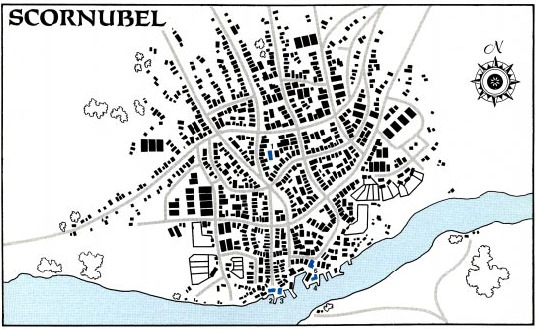
\includegraphics[height=7 cm, width= 9cm]{../Mappe/Scornubel.PNG.jpg}
\begin{itemize}
    \item \textbf{Tipo:} Città
    \item \textbf{Demonimo:} Scornubian o Scornubrian
    \item \textbf{Popolazione:} 14.000 nel 1479 DR
    \item \textbf{Governante:} Lady Rhessajan Ambermantle nel 1372 DR
    \item \textbf{Descrizione:} Situata sulla riva settentrionale del fiume Chionthar, dove la Trade Way raggiunge il fiume.
    \item \textbf{Trasporti fluviali:} 
    \begin{itemize}
        \item Barche, chiatte e skiff percorrevano il fiume fino a Baldur's Gate, Berdusk e Hill's Edge.
    \end{itemize}
    \item \textbf{Storia:} 
    \begin{itemize}
        \item La parte meridionale era un tempo la città rivale di Zirta.
        \item Dopo la Spellplague del 1385 DR, la città fu annessa a Elturgard.
    \end{itemize}
    \item \textbf{Governo:} 
    \begin{itemize}
        \item Governata da Lady Rhessajan Ambermantle.
        \item Consiglio di tre ex-mercanti e un'ulteriore assemblea di mercanti.
    \end{itemize}
    \item \textbf{Stile di vita:} 
    \begin{itemize}
        \item Molti edifici cambiavano proprietà rapidamente.
        \item Molti residenti dormivano all'aperto o nelle loro carovane.
    \end{itemize}
    \item \textbf{Problemi di sicurezza:} 
    \begin{itemize}
        \item Raid da parte di bugbear e hobgoblin in inverno.
        \item Presenza di ladri e doppelganger.
        \item Tolleranza verso creature come lamie e doppelganger.
    \end{itemize}
    \item \textbf{Luoghi importanti:} 
    \begin{itemize}
        \item \textbf{Edifici ufficiali:} Scornubel Hall, ufficio dei Red Shields, Free Traders of Scornubel.
        \item \textbf{Edifici religiosi:} Healing House of Lathander, High Holy House of Coin (1490s DR).
        \item \textbf{Commercio:} Mercato del pesce, ferry dock, Trail Lords HQ, vari commercianti e artigiani.
        \item \textbf{Taverne e locande:} Mother Minx's, The Nightshade, The Dusty Hoof, The Raging Lion, The Jester's Bells.
        \item \textbf{Strade principali:} Trade Way, Northstorm Street, Red Shields Road.
    \end{itemize}
    \item \textbf{Abitanti noti:} 
    \begin{itemize}
        \item Lady Rhessajan Ambermantle (sovrana)
        \item Angah Lalla (commerciante di oggetti curiosi)
        \item Laertilus (esperto di tesori perduti)
        \item Vaerum (Maestro Ladro, ex capo di una gilda locale)
    \end{itemize}
\end{itemize}


\subparagraph{Costa del fiume Reaching}
 \textbf{Bugbear o Goblin}



\subparagraph{Reaching Woods} 
Tempo di di attraversamento 4 giorni + 3 per il Darkhold  
\begin{itemize}
    \item \textbf{Tipo:} Foresta
    \item \textbf{Razze:} 
    \begin{itemize}
        \item Hobgoblin
        \item Centauri
        \item Hybsil
        \item Satiri
        \item Goblinoidi
        \item Umani
        \item Elfi
        \item Goblin
        \item Gnoll
    \end{itemize}
    \item \textbf{Descrizione:} Grande foresta nei Western Heartlands
\end{itemize}

\subparagraph{Geografia}
\begin{itemize}
    \item \textbf{Posizione:} 
    \begin{itemize}
        \item Est del fiume Chionthar
        \item Sud delle Trielta Hills
        \item Ovest delle Far Hills
    \end{itemize}
    \item \textbf{Divisione:} Separata dal fiume Reaching
    \item \textbf{Nomi alternativi:} 
    \begin{itemize}
        \item Northdark Wood
        \item Dusk Wood
        \item Reluvethel's Wood
    \end{itemize}
\end{itemize}
\textbf{Clima}
\begin{itemize}
    \item \textbf{Inverno:} 
    \begin{itemize}
        \item Temperature gelide
        \item Nevicate ogni 3-4 giorni
        \item Bufere improvvise
    \end{itemize}
    \item \textbf{Aree ombreggiate:} Rimangono ghiacciate per tutta la stagione
\end{itemize}
\textbf{Storia}
\begin{itemize}
    \item \textbf{1° secolo DR:} Casa della città di Talis, abitata dai Talfir
    \item \textbf{557 DR:} Tribù hobgoblin attaccarono Phalorm, ma furono fermate dalle infiltrazioni di Phalorm
    \item \textbf{1459 DR:} Elturgard scoprì santuari a divinità non approvate e isolò la foresta
    \item \textbf{1479 DR:} I gnoll sterminarono gli altri abitanti e iniziarono a cibarsi dei sopravvissuti
\end{itemize}
\textbf{Abitanti}
\begin{itemize}
    \item \textbf{6° secolo DR:} Tribù hobgoblin occupavano la foresta
    \item \textbf{14° secolo DR:} Abitata da centauri, hybsil e satiri druidi
    \item \textbf{1367 DR:} I goblinoidi invasero e schiavizzarono i centauri e i satiri
    \item \textbf{15° secolo DR:} Dominata dai gnoll, che tennero umani ed elfi come cibo
\end{itemize}

\begin{description}
    \item[Giorno 1:] Guadano il fiume senza alcuna difficoltà, pagando 1 moneta d'argento a testa, Far e Jack pagano per loro. Entrano nella foresta (Percezione CD 15) percependo qualcosa di strano nell'aria e che potrebbero essere osservati. Appena fermati, gli gnoll attaccano (il più lontano cerca di scappare se li massacrano).
    
    \item[Giorno 2:] Dopo l'attacco notturno, se lo gnoll è scappato, il nuovo attacco avviene a 3 ore dal risveglio, altrimenti si ritrovano di fronte la pattuglia (Percezione CD 12) per notarli. Far e Jack sono straniti dalla presenza di così tanti Gnoll anche di così alto rango. Se combattono, a terzo round o se sono in difficoltà, interviene un centauro (Norberto, parla solo Elfico e Silvano). Dopo aver combattuto, il centauro li invita a seguirlo dalla tribù degli hobgoblin.
    
    \item[Giorno 3:] Se hanno accettato, incontrano Yasbul capitano degli hobgoblin , con pochi soldati rimasti, invita tutto il gruppo ad unirsi all'attacco notturno, non hanno molto da offrire, ma sanno che se gli gnoll non verrano fermati potrebbero attaccare la città e causare più danni alla foresta. Se rifiutano, Far e Jack seguono il gruppo senza problemi. Se non hanno accettato, proseguono sulla loro via, ma durante il cammino vengono accerchiati dagli Gnoll. 
    
    \item[Giorno 4:] Se si sono uniti alla causa, allora arrivano direttamente al combattimento finale. Se non si sono uniti, continuano verso il Darkhold e poi Far e Jack andranno per conto loro.
\end{description}

\textbf{Gnoll Zanna di Yeenghou}: Sono gnoll benedetti/maledetti da un demone inviato dal signore degli gnoll Yeenoghu. E in genere la presenza di uno gnoll di questo tipo incrementa drasticamente la popolazione. 
        \section{IDEE}
            \begin{itemize}
                \item Usare la pagina 73 del manuale Guida agli avventurieri della costa
                \item Controllare il Percorso lungo il fiume
                \item Collegare la scomparsa di Sebine,  all'Animale che vuole usarla per ottenere un patto con "Nome diavolo", per far tornare  gli Zhentarim allo splendore di un tempo
                \item Il Darkhold è vasto, Necrov continua a sconsigliare di andare.
                \item Aggiungere un PNG che colleghi Grigarr (GACS) all'Animale
                \item Se vanno prima a cercare Alta Radiosità, scoprono che servono gemme da 1000 mo, Necrov passato un pó dark, ha agganci nel Darkhold.  
            \end{itemize}

\end{document}       